\documentclass[en,hazy,blue,screen,14pt]{elegantnote}
\usepackage[T1]{fontenc}
\usepackage[latin9]{inputenc}
% \usepackage[USenglish]{babel}
\usepackage{babel}
% TODO: interesting bug about the font of proof env
\usepackage{float}
\usepackage{textcomp}
\usepackage{amsmath,amsfonts,amssymb}
\usepackage{amsthm}
\usepackage{graphicx}
\usepackage[ruled,vlined]{algorithm2e}
\PassOptionsToPackage{normalem}{ulem}
\usepackage{ulem}
\usepackage{mathtools}
\usepackage{url}
\usepackage{hyperref}

\DeclarePairedDelimiter{\ceil}{\lceil}{\rceil}
\newcommand\tab[1][1cm]{\hspace*{#1}}
\newenvironment{claim}[1]{\par\noindent\underline{Claim:}\space#1}{}
\newenvironment{claimproof}[1]{\par\noindent\underline{Proof:}\space#1}{\hfill $\blacksquare$}

\title{Class Notes\\CIS 502 Analysis of Algorithm\\4-Greedy Algorithm}
\author{Da Kuang}
\institute{University of Pennsylvania}
%\version{1.00}
\date{}
%\pdfpkresolution=150    % dpi       % see pdftex manual

\begin{document}
	
\maketitle
\newpage

\section{Optimization Problem}
\begin{definition}
\textbf{Optimization Problem:} Minimize or maximize some function subject to 
some constrains.
\end{definition}

Now we start with a special class of optimization problem:

\begin{itemize}
 \item Given a set of elements, pick a subset.
 \item Constrains tell you which subsets are allowed.
 \item Any allowed subset is a feasible solution.
 \item Objective function assigns a value to every feasible solution.
 \item Goal is to find the feasible solution with greatest/ least value.
\end{itemize}
ddd

\subsection{Minimum Spanning Tree Problem}
Minimum spanning tree problem is an example of optimization problem.
\paragraph{Input:} Connected, undirected graph $G \in (V,~E)$ together with a 
weight function $w: E \rightarrow \mathbb{R}^+$.

\begin{definition}
 The \textbf{feasible solution} is a set of edges forming an acyclic connected 
graph on all vertices.
\end{definition}

\begin{definition}
 The \textbf{cost} of a solution is the sum of the weights of the edges in the 
solution.
\end{definition}

The are problems for which the optimal solution can be pick by choosing one 
element at a time.

\begin{definition}
The \textbf{greedy algorithm} builds up solution as by taking the next element 
to be one of the optimal cost value that can be added feasibly.
\end{definition}

Most of the time Greedy algorithm itself is simple but it is difficult to prove 
correctness.



\section{Activity Selection Problem}
\begin{itemize}
 \item \textbf{Input:} $n$ activities $a_1, \cdots, a_n$, where $a_i$ starts at 
time $x_i$ and ends at time $y_i$.
\item \textbf{Feasible Solution:} Any subset of these activities such that no 
two activities in the subset overlap. 
\item \textbf{Objective Function:} Maximize the number of activities we 
schedule.
\end{itemize}

\subsection{Some Attempts}
Criterions to be greedy on:
\begin{itemize}
	\item Pick the activities with shortest duration. 
	
	It dose not work. The counter example is as follows:
    \begin{figure}[H]
    \centering
    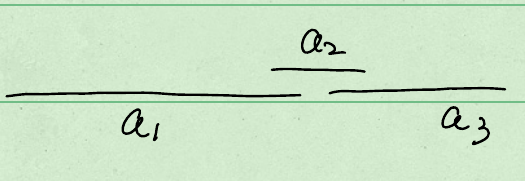
\includegraphics[width=0.3\textwidth]{1st-attempt.png}
    \end{figure}
	\item Pick the activities what finish first.\\
        Sort the activities by finish time and then renumber them so that $f_1 
\le f_2 \cdots \le f_n$
\end{itemize}
\subsection{Proposed Greedy Algorithm}
Given a set of activities, 
\begin{itemize}
	\item Pick the earliest finishing activities that remain.
	\item Remove all activities that conflict with the chosen activity.
	\item Repeat.
\end{itemize}

To prove the correctness, we start by arguing that the algorithm 
is not wrong on its first choice.

\begin{claim}
	\textbf{Greedy Choice Property:} First choice made by greedy algorithm is 
not wrong.
\end{claim}
To be more specific, in activities selection problem, if greedy algorithm 
choose an activity at first, then there is an optimal feasible solution that 
contain $a_1$.

\begin{claimproof}
	Suppose for contradiction that no optimal feasible solution uses $a_1$. 
Let $O$ be the subset of activities in some optimal solution. We can order the 
activities in $O$ by finish time.

    Let $a_{i1}, a_{i2}, \cdots, a_{ik}$ be the activities in $O$ so ordered. 
We can make an \textbf{exchange argument} as the following plot. Throw out 
$a_i$ from $O$ and include $a_1$ in instead to get a new set of activities 
$O'$. 

    There are some properties about $O'$.
    \begin{itemize}
        \item $|O'| = |O|$
        \item $O'$ is feasible.
        \item $O'$ is also optimal and contains $a_1$. 
$\Rightarrow\mskip-\thinmuskip\Leftarrow$
    \end{itemize}

    \begin{figure}[H]
    \centering
    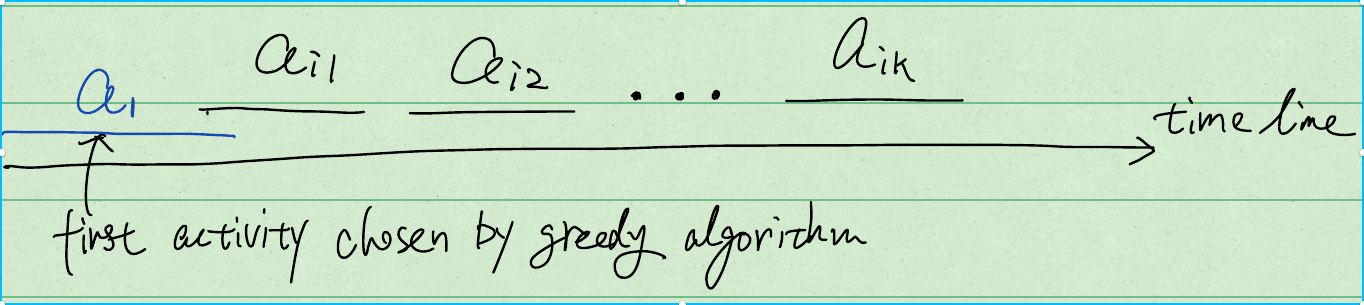
\includegraphics[width=0.5\textwidth]{exchange-selection-1.png}
    \end{figure}
\end{claimproof}

There is a way to construct an optimal solution starting with $a_1$. This 
optimal solution should certainly exclude activities that conflict with $a_1$. 
Recursively need to solve a smaller problem consisting of activities that do 
not conflict with $a_1$. In particular, the smaller problem is finding the 
optimal subset of activities out of the remaining activities.

\begin{claim}
    \textbf{Optimal Substructure Property}
	In the set of activities, we need to pick an optimal feasible 
subset activities.
\end{claim}
\begin{claimproof}{}
\begin{itemize}
	\item $A$: Original set of activities
	\item $A'$: Set of activities that remain after throwing out $a_1$ and 
its conflicting activities.
\end{itemize}
    Any solution to $A'$ that gives value $k$ can be extended to a solution to 
$A$ of value $(k+1)$ by adding $a_1$. So need optimal solution to $A'$
\end{claimproof}

In general. Optimal Substructure Property inductively assumes that greedy 
solves problem with fewer than $n$ activities optimally.

Greedy Choice Property and Optimal Substructure Property imply that greedy 
solve $n$-activity problem optimally.

\subsubsection{Time}
We sort the activities by finish time take $O(n\log n)$. Then the rest of steps 
can be done in linear or constant time.


\section{Linear Algebra}
\begin{definition}
	$V$ is a \textbf{vector space over $\mathbb{R}$} if
	\begin{itemize}
		\item For $v_1, ~v_2 \in V$, $v_1 + v_2 \in V$.
		\item For any $\alpha \in \mathbb{R}, ~v \in V$, $\alpha v \in V$.
	\end{itemize}
\end{definition}

\begin{definition}
    Given a finite set of vectors, $v_1, v_2, \cdots, v_k$, then \textbf{span} 
$S$ is as 
    follows
    \[S(v_1, v_2, \cdots, v_k) = \{v: v = \alpha_1 v_1 + \alpha_2 v_2 + \cdots 
    +\alpha_k v_k, ~\alpha_i \in \mathbb{R}\}\]
\end{definition}
$S(v_1, v_2, \cdots, v_k)$ is a vector space.

\begin{definition}
	$\alpha_1 v_1 + \alpha_2 v_2 + \cdots +\alpha_k v_k$ is a \textbf{linear 
combination} of vectors. 
\end{definition}

\begin{definition}
    The set of vector $v_1, \cdots, v_k$ is called \textbf{linear dependent} if 
there exist some coefficient $\alpha_1, \cdots, \alpha_k$ not all $0$, so that 
$\sum \alpha_i v_i = 0$
\end{definition}

\begin{definition}
	A set of vector is said to be \textbf{linearly independent} if it is not 
linearly dependent.
\end{definition}

\begin{definition}
	If $v_1, \cdots, v_k$ are linearly independent and their span in $V$, then 
$v_1, \cdots, v_k$ form a \textbf{basis} of $V$.
\end{definition}

\begin{definition}
	If $v_1, \cdots, v_k$ is a basis for $v$ and $u_1, \cdots, u_m$ is another 
basis. Then $m = k$.
\end{definition}

\begin{proof}
	Suppose for contradiction that $m > k$. Since $v_i$'s from a basis,
	\begin{align*}
		u_1 &= \alpha_{11} v_1 + \cdots + \alpha_{1k}v_k\\
		u_2 &= \alpha_{21} v_1 + \cdots + \alpha_{2k}v_k\\
            &\vdots\\
        u_m &= \alpha_{m1} v_1 + \cdots + \alpha_{mk}v_k\\
	\end{align*}
Will prove $(u_1, \cdots, u_m)$ is linearly dependent. Need to show
$\sum x_i u_i = 0$ for some $(x_1, \cdots, x_m)$ not all zero.
\begin{align*}
	&x_1 u_1 + x_2 u_2 + \cdots + x_m u_m = 0\\
	\intertext{substitue $u_i$ with $v_i$'s,}
	&(x_1 \alpha_{11} + x_2 \alpha_{21} + \cdots + x_m \alpha_{m1}) v_1\\
	+~& \cdots\\
	+~&(x_1 \alpha_{1k} + x_2 \alpha_{2k} + \cdots + x_m \alpha_{mk}) v_k = 0
\end{align*}
All the coefficients above should be 0. There are $k$ coeficientes, $m$ 
equations and we assume $m > k$. Therefore, there are infinite possible 
combinations of $x_i$'s. Therefore, there must be a solution which is not 
all zeros. Because if there is not such solution, then there should be only one 
solution which is all zeros.
\end{proof}




\section{Maximum Total Weight Problem}
Suppose you are Google and you assign a vector to each possible document. When
a user searches for a term, you want to collect some vectors that are indicative of that search term. You also want to be diverse, e.g., if a user searches for "jaguar" you want to return some documents with cars and others with the animal. We could model this by returning vectors that are linearly independent.

\begin{itemize}
	\item \textbf{Inputs:} vectors $(v_1, v_2, \cdots, v_n)$ with weights 
$(w_1, w_2, \cdots, w_n)$.
    \item \textbf{Goal:} Find a basis for the space spanned by $(v_1, v_2, \cdots, 
v_n)$ of maximum total weights.
\end{itemize}
\paragraph{Note.} A single vector is linear independent to any other vector if 
it is a zero vector.

\subsection{Greedy Algorithm}
\begin{itemize}
	\item Sort vectors and renaming them by descending order of weights.
	\item $S$ is an empty set of vectors initially.
	\item For each vectors $v_i$ in this order, if $S \cup \{v_i\}$ is linearly 
independent and $v_i$ is an non-zero vector, then $S = S \cup \{v_i\}$.
\end{itemize}

\subsection{Correctness}
\begin{theorem}
	\textbf{(Exchange Property)} Suppose A and B are finite subset of linearly independent vectors in $ \mathbb{R}^d $, and suppose $ |A| < |B| $. $\exists b \in B$, such that $ A \cup \{b\} $ in linearly independent.
\end{theorem}

\begin{proof}
	Indeed, there must be a vector in $ B $ that lies outside the space spanned by $ A $ because of the dimensions of space $ <B> $ and $ <A> $.
\end{proof}

\begin{theorem}
	\textbf{(Hereditary property)}. If $ R \subset S $ and $S$ is a linearly independent set of vectors, then $R$ is also linearly independent.
\end{theorem}

Greedy algorithm for finding a maximum of basis works because of vector has the exchange and hereditary properties.

\begin{itemize}
	\item Suppose greedy returns vectors $G = \{v_{i1}, v_{i2}, \cdots, v_{ik}\}$.
	\item Suppose, for contradiction, there is an optimal solution that return $O = \{v_{j1}, v_{j2}, \cdots, v_{jk} \}$, which has a better total of weights.
\end{itemize}

\begin{claim}
	$G$ is at least as good as $ O $.
\end{claim}
\begin{claimproof}
	
	Let $ v_{il} $ be the first vector chosen by greedy algorithm that is not in $O$. Let $ A = \{v_{i1}, \cdots, v_{il}\} $, $ B = O$. 
	
	Hence,
	\begin{itemize}
		\item If $ l = k $, $ G $ is at least as good as $ O $.
		\item If $ l < k $, $ |A| < |B| = k $. By exchange property, applied repeatedly, we can keep adding vectors from $ B $ to $ A $ while preserving linear independent to $ A $ until $ |A| = |B| $. In the end, after borrowing some elements from $B$, the only difference between $A$ and $B$ is that $ A $ has $ v_{il} $ instead of some vectors from $B$. Moreover, that vector has weight $ \le w_{il} $. So $ w(A) \ge w(O)$. The expanded list $A$ has a weight at least as good as $O$.
		
		What would be the relationship between $G$ and $A$.
		
		Note that even if $ w(A) = w(O) $, $ A $ still agrees more with greedy algorithm than $ O $. Suppose in the ``worest case'', no matter how to choose $l$, the weight of expanded $A$ always equal to the weight of $B$. We are still able to prove that greedy algorithm is as good as $ O $ by induction. So the claim still holds.
	\end{itemize}
	
%	Since the $v_j$'s form a basis,
%	\[v_{i1} = \alpha_1 v_{j1} + \alpha_2 v_{j2} + \cdots + \alpha_k v_{jk}\]
%	
%	$v_{i1}$ is chosen by greedy algorithm so it is not a zero vector. Therefore, 
%	there must be some $\alpha_l$ is non-zero.
%	
%	We can add $v_{i1}$ to the set $(v_{j1}, v_{j2}, \cdots, v_{jk})$ and kick out 
%	$v_{jl}$.
\end{claimproof}






\section{Find Maximum Spanning Tree}
\subsection{Maximum Weight Minimum Spanning Tree}
\textbf{Input}: a connected, weighted, undirected graph $ G = (V , E) $ with weight function $ w : E \to R $. 

\textbf{Goal}: Find a maximum weight spanning tree in $G$. 

Because this is the problem of finding a maximum weight of maximum independent set in a graphic matroid, the greedy algorithm is optimal.

\subsection{Kruskal's Algorithm}
\textbf{Main Idea}: Sort the elements in the ground set (edges) in decreasing order of weight and then repeatedly add edge as long as adding new edge keeping the graph acyclic.

\textbf{Consider}: Suppose Kruskal's algorithm has found the following edges, what makes the algorithm to decide to pick an edge?

Think in a shallow way. The new edge shall not create a cycle in the graph. To be more specific, if the vertices from the new edge belongs to the same component then it will introduce a cycle since vertices with in the component are already connected. Conversely, if the vertices come from different components then it cannot be a cycle.

So Kruskal's algorithm maintain the connected components it has discovered so far then includes edge $ (u, v) $ lie in different component before the inclusion.

\textbf{Remark}: So far we have focused on finding maximum spanning tree but it turns out that the greedy algorithm works for finding minimum spanning tree as well. The only difference is to sort the weights by descending order for minimum spanning tree. For minimum spanning tree, we can use the same greedy algorithms.

\subsubsection{Algorithm}
Kruskal's algorithm finds a minimum weight spanning tree in a connected, weighted, undirected graph.
\begin{itemize}
	\item Sort and renumber the edges in increasing order of weight as $ e_1 , \dots, e_n $.
	\item Maintain a graph G with the same vertices as the original graph to track the edges chosen already.
	\item When considering $ e_i = (u, v) $, add $e_i$ to the graph if and only if $u$ and $v$ lie in different components. To do this, we need two routines.
	\begin{itemize}
		\item Find operation: return the component for a vertex u.
		\item Union operation: merge two components together.
	\end{itemize}
\end{itemize}
We define a \textsc{union\_find} data structure for find and union operation. Initially no edge is chosen by the algorithm and every vertex is a component by itself. Therefore, we will initialize the data structure to $n$ singleton components.

Now we are going to explore some of the possible data structure to be used for \textsc{union\_find}.

\paragraph{Attempt 0.} Maintain the information in array. Make index of array is the vertex name and value is the name of the component.

For this structure, find operation is $\mathcal{O}(1)$. Union(u, v) = $\mathcal{O}(n) $, since in worst case you may have to rename all the vertices. In the course of Kruskal's algorithm, $n-1$ union operations to perform. So this is a rather expensive design choice.

\paragraph{Attemp 1.} Suppose $u$'s set contains $n_1$ elements and $v$'s set contains $n_2$ elements. 

When Union-ing two sets, change the name for the elements in the \textbf{smaller} sets. But in the worst case, the union still takes $n$ steps. Moreover, even in a good case, there is only one element in a set but we still need to scan the whole list to know the size of set. Therefore, we introduce a new array to maintain a linked list for each set containing the elements in that set.

Remark: The array is used to from vertex to set and set is used to find the vertices of each set.

Even with the help of new linked list, an individual union operation could still take $\Theta(n)$ steps. However, we can use \textbf{amortized analysis} to make the our analysis more tight by looking at the whole sequence instead of single operation. In fact, any \textbf{sequence} of $k$ union operations performed by Kruskal's algorithm take only $\mathcal{O}(k\log n)$ steps.

\subparagraph{Amortized Analysis.} In computer science, amortized analysis is a method for analyzing a given algorithm's complexity, or how much of a resource, especially time or memory, it takes to execute. The motivation for amortized analysis is that looking at the worst-case run time per operation, rather than per algorithm, can be too pessimistic. The target of amortized analysis is rather special since it is neither average nor worst case.

For example, suppose given two sets A and B, the goal is to calculate the union of the sets. It is known that the cost of operation is $|B| = n$.
 
Accounting method is used for analysis:
\begin{itemize}
	\item Set up an account for each element in the data structure. 
	\item Charge 1 to each element in the smaller set for a union operation. 
	\item Every time an element is charged. It joins a set at least twice as large. \\ $\rightarrow$No element is charged more than $\log n$ times.
\end{itemize}

Therefore, the total cost of a sequence of ($n-1$) union operations to union $A$ and $B$ is at most $n \log n$. (With some most carefully analysis, $k$ union cost at most $k\log k$. But $n\log n $ is good enough for the course.)

\paragraph{Attemp 2.} Maintain connected components in a tree so that we have a forest as follows. The name of the component is the element at the root. The name of each vertices are saved in the array of leaves. For each leaf in the tree, keep a pointer to its parent. 

\begin{figure}[H]
	\centering
	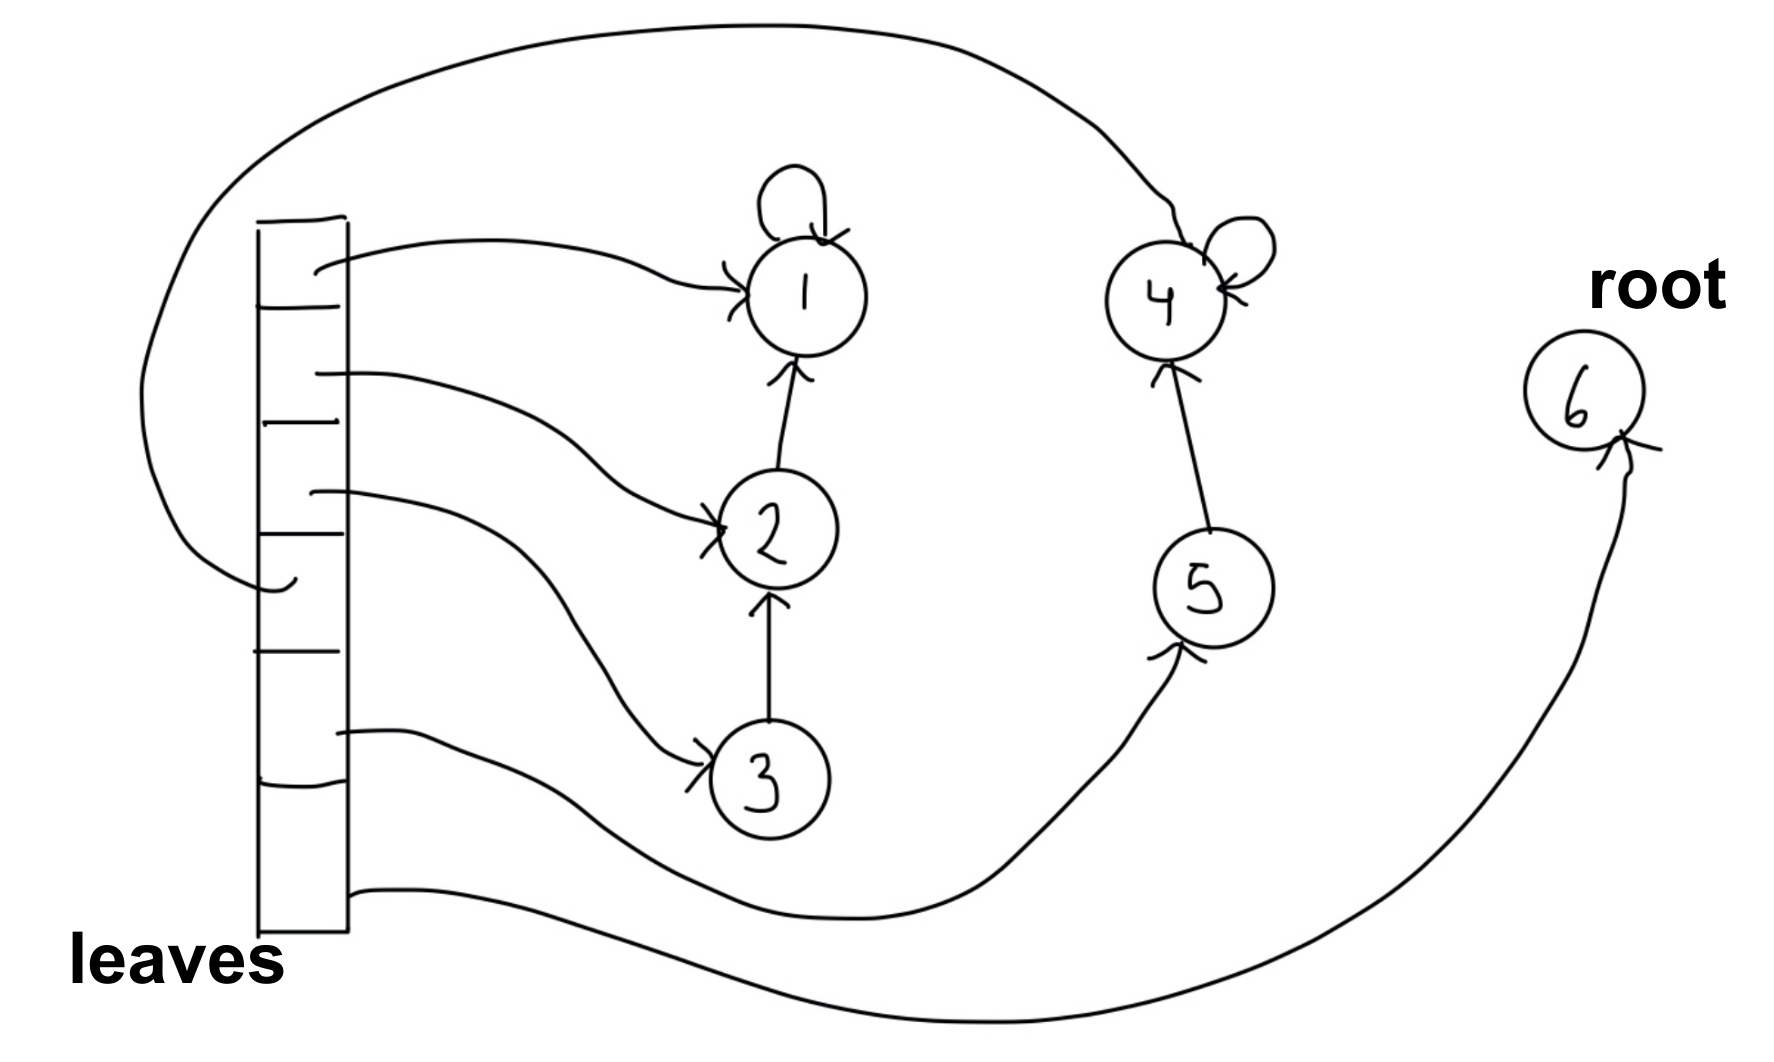
\includegraphics[width=0.5\textwidth]{attemp-2.png}
\end{figure}

\subparagraph{\textsc{Find}.} Traverse up the tree by the pointer until you find the end of linked list, which is a root and you will have found the component of the vertex. Hence, \textsc{Find} cost a proportion of the height of the tree. 

\subparagraph{\textsc{Union}.} \textsc{Union} make one root point to the other. 
%Make the root of the tree with pure elements prompt up to the root of the other tree. 

How to find the time complexity of each operation? We can do the same optimization trick like in Amortized Analysis. We make the root of the smaller tree point to the root of the larger tree. Based on that, we claim that all tree heights at all times are $ O(\log n) $.
\begin{claimproof}
	Think about any element in any of the trees, when the cost for it passes through the root increase by 1? After the tree unions with other tree, in which case the size of the sets increases at least by twice. Therefore, no element can be more than $O(\log n)$ away from the root.
\end{claimproof}

Therefore, we have the confidence to claim that \textsc{Find} operations are $ O(\log n) $ in the worst-case. The \textsc{Union} operations of arbitrary pairs of elements are also $ O(\log n) $.

Recall that $|E| = m$ and $|V| = n$. Kruskal's algorithm does $O(m)$ find operations and $O(n)$ union operations. So overall, $O(m \log n)$ steps for all union and find operations. Note that sorting edges at the beginning already takes $O(n\log n)$ steps. (? Here it should be $O(m\log m)$, but $O(m\log m) = O(n\log n)$?) So far \textsc{union\_find} is not the sole bottleneck since it has the same time complexity with sorting. 

But still, there is one more optimization for \textsc{Union} operation even though it will not help to improve the overall performance of Kruskal's algorithm.

\paragraph{Path Compression.}
First, let's reflect on one of the features of the tree we just build. 

Unlike with the common tree structures, here we start from any internal node pointing by the pointer and then go upward from the child to its parent. 

In the common tree (binary search tree, heap tree), we have to limit the number of children because it will cause the traversal order problem and increase the complexity of the problem.

By controversial, the path in our bottom has deterministic direction. Moreover, like always, the height of the tree is the number of operations for solving problem. Therefore, we would keep the tree as much bushy and short as possible to reduce the number of operations.

Now motivated by making the tree bushy and short, we can do path compression as follows:

When doing \textsc{find}($u$), for each node encountered on the path from leaf $u$ to the root, make it a child of the root.

Note that path compression could not improve the worst case time of either \textsc{find} or \textsc{union}. But it gives a great amortized complexity. Any sequence of $m$ starting from the initial \textsc{union-find} data structure on elements takes at most $O(m\log^*n)$ time.
\begin{definition}
	$\log^*n$ is a really really slow function which almost like a constant. It is the number of times you need to take $\log$ to get $n$.
\end{definition}
For example. $\log^* 16 = 3$. $\log^* (2^{16} = 65536) = 4$. $\log^* (2^{65576} = 65536) = 4$

We did not cover the analysis of path compression during class.
\subsection{Prim's Algorithm}
Prim's algorithm is another greedy algorithm for finding a maximum weight spanning tree. In the canonical greedy algorithm, we keep adding edge one at a time but how to select the right edge in the graph? Here we introduce a concept \textbf{cut.}

\begin{definition}
	A \textbf{cut} in a graph $G = (V, E)$ is defined by non-trivial partition $ V_1 \cup V_2 $ of $V$. The cut $ (V_1, V_2) $ is a set of edges that have exactly one end point in $ V_1 $.
\end{definition}

\begin{claim}
	For $e \in \text{cut}(S, V-S)$, if $e$ is the heaviest edge in the set. Then it will not cause a cycle with other edges have been connected by greedy algorithm. Therefore $e$ will be included in the maximum weighted independent set.
\end{claim}
\begin{claimproof}
	By the canonical algorithm of greedy algorithm, we consider edges in decreasing order of weights. By the time we consider the edge $e$, we have not consider any other edge cross the two sets of the cut yet since $e$ has the largest weight. Therefore, $e$ will not cause any cycle with the edges that the greedy algorithm has chosen. Because you need two edges cross the two components to get a cycle.
\end{claimproof}

Prim's algorithm is one specialization of this idea that if you can find the heaviest edge in each cut then you can build a minimum spanning tree. Prim's algorithm consider a particular set of cuts.

\textbf{Main Idea}: Split the graph into two sets $S$ and $V-S$. Some vertex $s$ is arbitrarily chosen as the initialization of $S$. First consider the cuts consisting $s$. Find the heaviest edge $(s, v)$. Bring $v$ into set $S$. Repeat the steps for the next heaviest cutting edge.

\subsection{Algorithm}
Initially, 
\[
d(v) = 
\begin{cases}
w(s, v) \text{, if $(s,v) \in E$}\\
\infty \text{, otherwise}
\end{cases}
\]
For each $ v \in V-S $, maintain $ d(v) $, weight $ \mathfrak{I} $ and the lightest edge $(x, y)$ from $V-S$ to any source vertex $x$ in $S$.

At each iteration, when we move the vertex $y$ that has the cheapest
edge to a vertex in $S$, we need to update every neighbor $v$ of $y$ so that $ d(v) = \min(d(v), w(v, y)) $.
\begin{figure}[H]
	\centering
	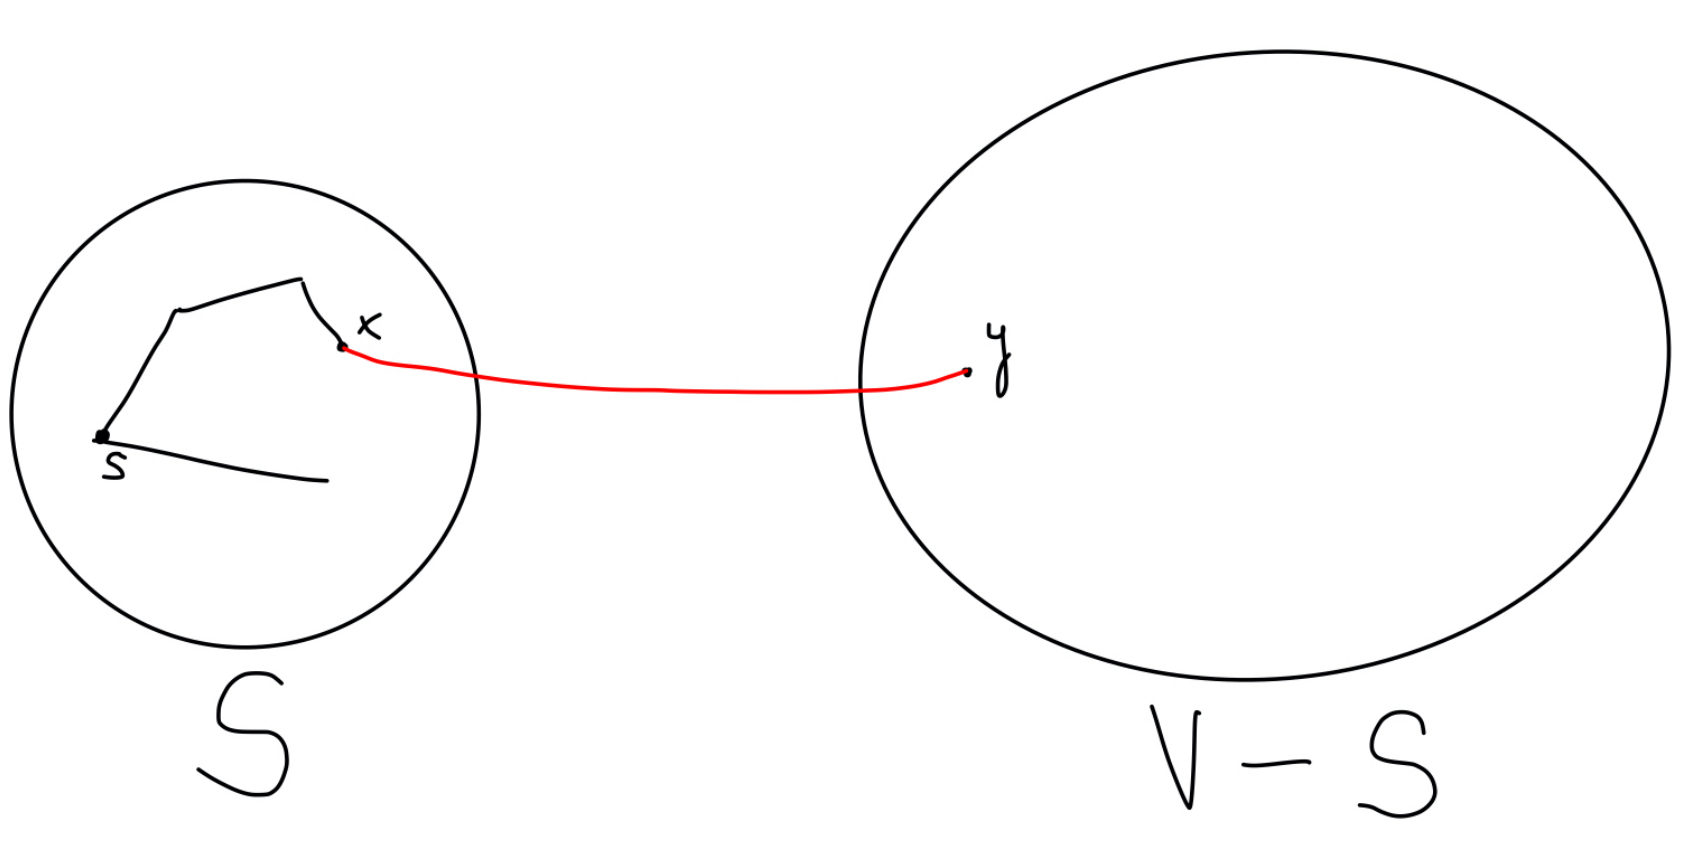
\includegraphics[width=0.5\textwidth]{prim.png}
\end{figure}

\subsection{Time Complexity}
If we maintain the $ d(v) $s in an array $ A $, the complexity is $ O(n^2) $ because we need to first find the minimum in $A$, and once we've found the minimum we need to update all the neighbors of the minimum.

If we maintain the $ d(v) $s in a min-heap, the complexity is $ O(m log(n)) $. Usually $m \le n$.


















\section{Shortest Path}
 Directed, weighted graph $G = (V, E)$with weight function $w: E \rightarrow \mathbb{R}$.
 
 Note that the algorithm can work on undirected graph as well since undirected graph can be seen as a special directed graph. So a undirected graph problem can be reduced to a directed graph problem but not necessarily vice versa. Moreover, the world is full of directed graph (download/upload speed, railway direction). The directed graph is a more general problem. 

There are two common sub-problem about the shortest path:
\begin{enumerate}
	\item Single source shortest path: Find the shortest path from a given vertex $s$ to all other vertex.
	\item All-pair shortest path: $\forall u, v,$ find length of the shortest path from $u \rightarrow v$.
\end{enumerate}
In most of the time, other problem can be reduced to these two problems. For example, single destination shortest path problem can be seen as a single source shortest path problem on the reversed graph.

Notice that there is actually no particularly better algorithm to solve single-source-single-destination problem. To find the shortest path from $s$ to $t$, the best we can do is to find the shortest path from $s$ to all the rest of the vertices. (TODO: This was a worst case example?)

\begin{definition}
	\textbf{The length of a path} is the sum of weights of all the edges on the path.
\end{definition}

 \subsection{Single Source Shorest Path}
Note: there is no matroid in the graph to solve the problem by greedy algorithm.

\subsubsection{Dijkstra's Algorithm}
\begin{itemize}
	\item Input: Directed Graph $G = (V, E)$ and a source vertex $s$.
	\item Assumption: all edge weights are non-negative (for example, driving time of the edges, latency of the internet, cost of putting a pipe).
	\item Goal: Find the shortest path from $s$ to all the vertices.
\end{itemize}

Maintain a quantity called $d(v)$ for each vertex $v$ so that,
\begin{itemize}
	\item $d(v)$ is an upper bound on the length of the shortest path from $s$ to $v$.
	\item There is a path from $s$ to $v$ of length $d(v)$.
\end{itemize}

Based on the assumption, we know that the shortest path from $s$ on the graph is to $s$ itself. We maintain a source set $S$ initially as $\{s\}$ and we know the shortest path form $s$ to each $u \in S$. Grow $S$ until $S = V$. Then we know the shortest path from $s$ to all the vertices.

A path from $s$ that stay eventually within $S$ will be called a source-side path.

\paragraph{Main idea}
At each state, find a vertex $v \in (V-S)$ for which there is a vertex $u$ in $S$ such that $d(s, u) + w(u, v)$ is minimum over all $x \in (V-S)$. Add $v$ to $S$. Update as appropriate.

\paragraph{Algorithm} 
\begin{itemize}
	\item For each vertex $v \in (V-S)$, maintain a quantity call $d(v)$. It is the length of the shortest path from $s$ to $v$ which consist of a source side path to a some vertex $u in (V-S)$ followed by edge $(u,v)$.
	\item In each iteration, bring the vertex $v$ with minimum $d(v)$ to $S$. To make sure $d$ is invariant, we have to update $d$ based on the new $S$ (with a new vertex $v$). For each neighbor vertex $x$ of $v$, update $d(x) = \min(d(x), d(v) + w(v, x))$. Note that if $v$ is used to update $x$, then we remember $v$ as the ancestor of $x$.
\end{itemize}

\subsubsection{Correctness}
\textbf{Statement}: For each vertex $v \in S$, $d(v)$ is equal to the length of the shortest path from $s$ to $v$.

This statement proves the correctness of the algorithm, since when $S = V$, we have the shortest path from $s$ to all the vertices.

\begin{proof}
	Initialization: $d(s) = 0$, $d(v) = \infty$ for $\forall v \neq s$.
	
	Prove the statement by induction.
	\begin{itemize}
		\item \textbf{Base case}: After the first iteration, $S = \{s\}$ and $d(s) = 0$, which is correct.
		\item \textbf{Inductive Hypothesis}: Assume the statement is true for $|S| = k$. Suppose $v$ is the $(k+1)$-th vertex brought to $S$. $v$ has $\min(d(v))$.
		\item \textbf{Inductive Step}: Let it call the path with length $d(v)$ as $P$. For contradiction, suppose there is a shortest path $P'$ to $v$. $P'$ must include at least one edge from $S$ to $(V-S)$. Let $(x, y)$ be the first such edge. Then the $(s, y)$ portion of $P'$ is already at least as long as $P$ by the way algorithm works. We get a contradiction by assuming the existence of $P'$.
		
		This proves that at the point the algorithm brings $v$ into $S$, $d(v)$ is the length of the shortest path to $v$. So we complete the induction.
	\end{itemize}
\end{proof}

Why negative weight does not work here?

Adding a negative edge into source set can change the length of shortest source-side path for some vertices. But we do not update $d(u)$ for $u \in S$ since we assume introducing more notes on the path only increase the length of path.

\section{Huffman Coding}
Given a text, which is a string over a large alphabet (say as English Text), we need to encode the text in binary for storage and communication.

Goal: Minimize the length of the binary code of the text.

Related problem: Code has to be a mapping from symbols in the original alphabet, $\Sigma$, to binary string.

\subsection{Prefix-ambiguity}
If one coded word is a prefix of another, then that could lead to ambiguity. Therefore, code must be ``prefix free'', which are called \textbf{prefix code}.

Ideally, we could like to assign shorter code to the words with higher frequency.
\subsection{Algorithm}
Input: $\Sigma = \{\sigma_1, \sigma_2, \cdots, \sigma_n\}$. $f_i$ is the frequency of $\sigma_i$. Assume that $\sum f_i = 1$, $f_i \ge 0 \forall i$.

Goal: Find a prefix code that makes $\sigma_i$ to $c(\sigma_i)$ to minimize $\sum f_i(\sigma_i)$, which is the average code length.

\end{document}
